\newpage
\section{CRC}

CRC kĩ thuật được ứng dụng trong việc kiểm tra lỗi của dữ liệu nhận được. Trong trường hợp đường truyền của bạn hay gặp nhiều nhiễu như ứng dụng điều khiển động cơ công suất lớn, có thiết bị chuyển mạch như relay hoặc fet đóng cắt dòng cao, hoặc đường truyền theo chuẩn RS-485 truyền đi quãng đường xa\dots dữ liệu của bạn trong khi truyền đi trên đường truyền có thể bị biến đổi và khiến hệ thống hoạt động sai.

Việc đề cập chi tiết tới giải thuật nằm ngoài phạm vi của tài liệu này. Các bạn có thể tham khảo ở đường link: http://www.sunshine2k.de/articles/coding/crc/understanding\_crc.html. Ở đây mình sẽ hướng dẫn bạn cách sử dụng nó cho ứng dụng của mình.

Phương pháp của CRC là nó sẽ dựa trên dữ liệu bạn sắp truyền, tính toán toán ra một con số 8-bit, 16-bit hoặc 32-bit. Con số này sau đó sẽ được truyền theo sau dữ liệu của bạn. Ở phía nhận dữ liệu sẽ tính toán lại một lần nữa dữ liệu mà nó nhận được, so sánh với số CRC mà bên gửi đã gửi kèm theo, nếu bằng nhau thì coi như dữ liệu nhận được là chính xác.

\begin{figure}[h!]
	\centering
    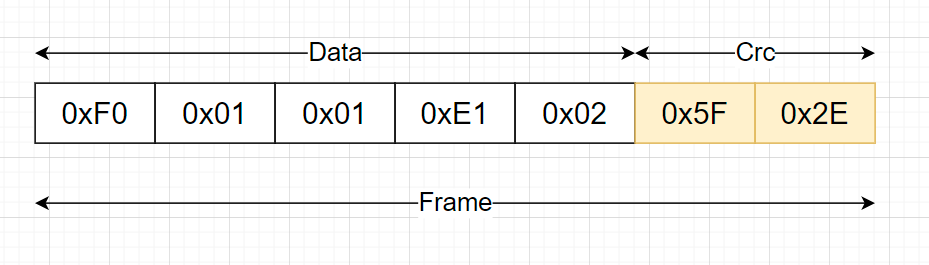
\includegraphics[width=\textwidth]{CRC.PNG}
\caption{Data frame with CRC}
\end{figure}

Các phần trình bày ở trên đã có phần demo. Còn trong trường hợp dự án thực tế cần cả 3 kĩ thuật slip, ring buffer và crc để đạt độ tin cậy tối đa khi chương trình chạy. Phần demo cho việc kết hợp cả 3 kĩ thuật này vào một project mong bạn đọc tự làm cho mình.